\documentclass[a4paper, 11pt]{report}

\usepackage[utf8]{inputenc}
\usepackage[french]{babel}
\usepackage{eurosym}
\usepackage{graphicx}
\usepackage{titlesec}
\usepackage{listings}
\usepackage{color}
\usepackage[french]{cleveref}
\usepackage{parskip}
\usepackage{tikz}
%%\usepackage{hyperref}
\usepackage{minitoc}


\definecolor{dkgreen}{rgb}{0,0.6,0}

\newcommand{\sectionbreak}{\clearpage}
\newcommand{\pir}[0]{\textbf{$\pi r^2$}\xspace}
\newcommand{\coq}[0]{\textbf{Coq}\xspace}
\newcommand{\coqdoc}[0]{\textbf{Coqdoc}\xspace}
\newcommand{\yrg}[0]{\xspace\textbf{Yann Régis-Gianas}\xspace}
\newcommand{\epita}[0]{EPITA}
\newcommand{\lc}[0]{$\lambda$-calcul\xspace}

\crefname{lstlisting}{listing}{listings}
\Crefname{lstlisting}{Listing}{Listings}

\lstset{language=Caml, frame=single, language=Caml,
commentstyle=\color{dkgreen}, basicstyle=\ttfamily\footnotesize}
\lstset{literate=%
  {é}{{\'e}}1
  {è}{{\`e}}1
  {â}{{\^a}}1
}

\title{Rapport de stage de fin de tronc Commun: \\
  Réécriture de Coqdoc}
\author{François Ripault}
\date{FIXME}

\begin{document}

\renewcommand{\labelitemi}{$\bullet$}
\renewcommand{\labelitemii}{$\cdot$}
\renewcommand{\labelitemiii}{$\diamond$}
\renewcommand{\labelitemiv}{$\ast$}

\dominitoc
\begin{titlepage}
\begin{center}
\textsc{\Large Rapport de stage de fin de tronc commun EPITA}

\vfill

\rule{\linewidth}{0.5mm} \\[0.4cm]
{\huge \bfseries Refonte du logiciel Coqdoc}
\rule{\linewidth}{0.5mm} \\[1.5cm]

\begin{minipage}{0.4\textwidth}
\begin{flushleft} \large
\emph{Auteur :}\\
François Ripault \\
\small
\texttt{francois.ripault@epita.fr}
\end{flushleft}
\end{minipage}
\begin{minipage}{0.4\textwidth}
\begin{flushright} \large
\emph{Maître de stage :} \\
Yann Régis-Gianas
\small
\texttt{yrg@pps.univ-paris-diderot.fr}
\end{flushright}
\end{minipage}

\vfill

\fbox{
\begin{minipage}{\textwidth}
\underline{Résumé :}
L'INRIA travaille sur le projet Coq, un assistant de preuve. Au sein de ce
projet, le sujet de ce stage consiste en la refonte du logiciel de
documentation Coqdoc.
L'objectif est de le rendre plus extensible, plus facilement maintenable et mieux l'intégrer au sein
du projet.
\end{minipage}
}

\vfill
Stage effectué à \textbf{L'INRIA} du : 3 Septembre 2012 au 11 Janvier 2013

\begin{figure}[h]
\begin{tabular}{ccccc}

\includegraphics[scale=0.8]{../data/inria.jpg} & &

\includegraphics{../data/pps.png} & &

\includegraphics[scale=0.8]{../data/epita.jpg}
\end{tabular}
\end{figure}

\end{center}
\end{titlepage}

\thispagestyle{empty}

\tableofcontents
\thispagestyle{empty}

\setcounter{page}{0}
\chapter{Introduction}
  %% 3 -> 5 pages
  Le présent rapport détaille travaux effectués au cours du stage de fin
  de tronc commun à l'\epita, réalisé du 3 Septembre 2012 au 11 Janvier 2013.

  Le sujet du stage consiste en la refonte complète du logiciel de
  documentation \coqdoc.

  \section{Contexte du stage}
  Ce stage s'est déroulé au sein de l'INRIA, plus particulièrement dans
  l'équipe \pir.

  L'INRIA est l'institut national de recherche en informatique et en
  automatique. C'est un établissement public à caractère scientifique et
  technologique, qui est l'acteur principal de la recherche en informatique en
  France.

  Je fus intégré à l'équipe \pir{} appartenant au laboratoire Preuves, Programmes et
  Systèmes.

  Le laboratoire \textbf{Preuve, programmes et systèmes} est une unité mixte
  de recherche, rattachée à plusieurs établissements scientifiques (INRIA,
  CNRS, et l'université Paris Diderot), qui regroupe à la fois des
  chercheurs en informatique et en logique mathématique, au sein d'une même
  thématique, celle des langages de programmation, des systèmes distribués,
  et de leurs fondements logiques.

  Au sein de ce laboratoire, l'équipe \pir se concentre sur la recherche
  autour de la correspondance entre preuves et programmes, ayant donné
  naissance à l'assistant de preuves \coq, et le formalisme qui sous-tend
  l'implémentation d'un tel logiciel.

  Ce stage fut effectué sous la direction de \yrg, maître de conférence à
  l'université Paris Diderot, et chercheur au sein du laboratoire \pir.
  %% FIXME

  \section{Problématique du stage}
  L'objectif de ce stage est de refaire le logiciel de documentation de
  l'assistant de preuves \coq, ne répondant plus aux attentes de ses
  utilisateurs.
  En effet, bien que celui-ci remplisse correctement sa tache il souffre d'un
  manque crucial d'extensibilité et s'intègre mal dans la suite d'outils
  fournie avec \coq. Il s'agit donc de refaire entièrement \coqdoc{} afin de
  mieux l'intégrer dans \coq, tout en concevant une architecture qui permette
  de l'étendre facilement par la suite.

  \section{Motivations et perspectives}
  Le stage offre des perspectives très intéressantes en relation directe
  avec mes objectifs professionnels, tout en mettant en application les
  compétences que j'ai acquises au cours du cycle de tronc commun.
  %%% FIXME

  \subsection{Validation des acquis de tronc commun}
  Le projet proposé met en jeu des compétences propres au métier d'ingénieur.
  En effet, la conception d'un nouveau logiciel est en relation directe
  avec les enseignements de l'\epita:
  \begin{itemize}
    \item \textbf{Conception d'un logiciel:} le stage a pour but la réécriture à
      neuf d'un logiciel préexistant: \coqdoc. L'objectif est de créer un outil
      s'intégrant bien dans la suite \coq, palliant aux problèmes de l'outil
      précédent, mais également en réutilisant les éléments intéressants pour
      la nouvelle version de \coqdoc.

      La conception d'un nouveau logiciel permet de mettre en application
      les compétences de programmation mais également des aspects
      annexes concernant le développement de projet, telle que
      la documentation du code ou la réalisation de tests unitaires.
    \item \textbf{Gestion de projet:} Écrire un nouveau logiciel
      apporte également des problématiques concernant la gestion de
      ce projet: il faut choisir un cycle de développement
      approprié permettant dans le temps du stage, de réaliser
      l'application. Il s'agit également de répondre aux attentes
      des utilisateurs concernant le projet, et de faciliter l'intégration
      du logiciel au sein de la suite d'outils \coq.
  \end{itemize}

  \subsection{Introduction au monde de la recherche}
  Ce stage représente également une bonne introduction aux problématiques
  de recherche abordées dans le domaine de l'équipe \pir.

  En effet, bien que le sujet de stage mette en jeu des compétences surtout
  liées au domaine de l'ingénierie, le contexte scientifique du stage me
  permet de découvrir les problématiques de recherche dans le laboratoire PPS
  et plus particulièrement l'équipe de recherche \pir.

  Cela répond directement à mes objectifs professionnels puisque après l'\epita,
  j'ai l'intention de poursuivre dans le monde de la recherche. Ce stage me
  permet donc de valider cet objectif professionnel, tout en tissant des liens
  avec les scientifiques travaillant dans ce domaine.

  \section{Phases de déroulement et introduction du rapport}
  Ce rapport retrace les différentes phases de déroulement du stage :
  \begin{itemize}
    \item la prise de connaissance des problématiques à résoudre
    \item la conception du logiciel de documentation
    \item l'implémentation de ce logiciel \\
  \end{itemize}

  Une première partie présentes les différentes structures au sein desquelles
  s'est effectué mon stage, ainsi que l'intégration des réalisation de ce stage
  dans les travaux de l'entreprise.

  Dans une deuxième partie, nous analysons l'existant et définissons la méthodologie
  et les objectifs du stage.

  La troisième partie détaillera la phase de réalisation technique.

  Enfin, dans une dernière partie, nous offrons une analyse critique des
  résultats de ce stage.

\chapter{Présentation de l'entreprise}
%% 5 -> 10
  Le stage proposé s'est fait au sein de l'équipe \pir, appartenant au
  laboratoire PPS, regroupant des chercheurs de plusieurs instituts de
  recherche. Cette section présente l'institut de recherche qui m'a employé
  ainsi que le laboratoire PPS, pour enfin présenter l'équipe \pir.
  \section{Le secteur d'activité}
  L'INRIA est un acteur majeur de la recherche informatique, aussi bien en
  France qu'à l'international.

  Les activités de recherche de l'INRIA sont regroupées en 5 thèmes qui visent
  à décrire une \textbf{activité scientifique} très large :
  \begin{itemize}
    \item Mathématiques appliquées, calcul et simulation
    \item Algorithmique, programmation, logiciels et architectures
    \item Réseaux, systèmes et services, calcul distribué
    \item Perception, cognition, interaction
    \item STIC pour les sciences de la vie et de l'environnement \\
  \end{itemize}

  L'INRIA travaille avec de nombreux \textbf{partenaires industriels}.
  Les principaux partenaires sont les suivants :
  \begin{itemize}
    \item Alcatel-Lucent
    \item EDF R\&D
    \item STMicroelectronics
    \item Bull
    \item Andra
    \item Microsoft-research \\
  \end{itemize}

  L'institut ne se contente pas uniquement de collaborations avec l'industrie,
  c'est également un créateur \textbf{Start-up}, qui commercialisent des
  produits issus des prototypes de recherche, et du savoir-faire de l'INRIA

  L'INRIA possède également de nombreux \textbf{partenariats à
  l'international}, tant avec des universités mondialement reconnues qu'avec
  des sociétés multinationales.

  \section{L'entreprise}
    \subsection{Présentation générale}
    La fondation d'INRIA remonte à 1967 sous le nom de IRIA (Institut de
    recherche en informatique et en automatique). L'IRIA est devenu l'Institut
    national de recherche en informatique et en automatique (INRIA) en 1979.
    L'INRIA est placé sous la double tutelle du ministère de la recherche et
    du ministère de l'économie, des finances et de l'industrie. \\
    INRIA est signataire du Pacte PME depuis le 17 décembre 2008, et l'institut
    participe à l'espace européen de la recherche à travers le consortium
    ERCIM\footnote{Consortium de recherche européen pour l'informatique et les mathématiques}, dont il a été l'un des membres fondateurs en 1989.

    L’INRIA a pour vocation d’entreprendre des recherches fondamentales et
    appliquées dans les domaines des sciences et des technologies de l’information
    et de la communication (STIC). L’institut assure également un fort
    transfert technologique en accordant une grande attention à la formation
    par la recherche, à la diffusion de l’information scientifique et
    technique, à la valorisation, à l’expertise et à la participation à des
    programmes internationaux. Jouant un rôle fédérateur au sein de la
    communauté scientifique de son domaine et au contact des acteurs
    industriels, l’INRIA est un acteur majeur dans le développement des STIC en
    France.

    L’INRIA est actif au sein d’instances de normalisation comme l’IETF\footnote{Internet engineering task force},
    l’ISO\footnote{Organisation internationale de normalisation} ou le W3C\footnote{Worldwide web consortium} dont il a été le pilote européen de 1995 à fin 2002.
    Enfin l’institut entretient d’importantes relations internationales : en
    Europe, l’INRIA s’implique fortement dans le 6ème PCRDT\footnote{Programme Cadre de Recherche et Développement Technologique} où il participe
    à plus de 40 actions ainsi que dans le consortium ERCIM, qui regroupe 17
    organismes de recherche. A l’international, l’institut collabore avec de
    nombreuses institutions scientifiques via plusieurs laboratoires de
    recherche conjoints (LIAMA\footnote{Laboratoire Franco-Chinois
    d'informatique, d'automatique et de mathématiques appliquées}, PPS), les
    équipes de recherche associées,
    et différents programmes de coopération.

    \subsection{Les missions de l'INRIA}
    Les grandes missions de l'INRIA se résument dans les points suivants:
    \begin{itemize}
     \item Concevoir et maîtriser les futures infrastructures des réseaux et
     des services de communication
     \item Développer le traitement des informations et données multimédia
     \item Garantir la fiabilité et la sécurité des systèmes à logiciel
     prépondérant
     \item Coupler modèles et données pour simuler et contrôler les systèmes
     complexes
     \item Combiner simulation, visualisation et interaction
     \item Modéliser le vivant
     \item Intégrer pleinement les STIC dans les technologies médicales
    \end{itemize}
    \subsection{Organisation}
    L'organisation de l'INRIA est établie par le décret du 2 août 1985.
    L'institut est dirigé par un conseil d'administration, dont son
    président, assure également les fonctions de directeur général.
    Il peut s'appuyer sur les compétences de deux instances scientifiques :
    \begin{itemize}
      \item \textbf{le conseil scientifique}, instance de réflexion et de
      proposition de l'institut en matière de politique scientifique,
      \item \textbf{la commission d’évaluation}, instance chargée de procéder à
      l'évaluation des équipes de recherche et des personnels scientifiques
      et qui contribue à définir les orientations des activités de l'institut.
    \end{itemize}

    Le conseil d'administration regroupe :
    \begin{itemize}
      \item \textbf{Un membre de droit} : le directeur général du Centre national de
        la recherche scientifique ou son représentant.
      \item \textbf{7 représentants de l'état désignés} respectivement par les
        ministres chargés de la recherche, de l'industrie, du budget, de
        l'enseignement supérieur, de la défense, des relations extérieures et
        des télécommunications.
      \item \textbf{8 personnalités} : deux personnalités de l'industrie de
        l'informatique et de l'automatique, deux personnalités scientifiques,
        deux personnalités représentatives du monde du travail, deux
        personnalités choisies parmi les utilisateurs de l'informatique et de
        l'automatique désignées par le ministre chargé de l'industrie.
      \item \textbf{4 représentants du personnel} de l'institut ou leurs
        suppléants dont deux chercheurs, élus pour une durée de quatre ans
        renouvelable une fois, selon des modalités fixées par arrêté du
        ministre chargé de la recherche et du ministre chargé de l'industrie. \\
    \end{itemize}

    \subsubsection{L'INRIA en chiffres}
    L'INRIA est structuré en 6 unités de recherche à travers la France :
    Rocquencourt et son antenne Parisienne, Rennes, Sophia Antipolis, Grenoble,
    Nancy, Bordeau, Lille, Saclay, Marseille, Lyon et Metz. \\

    En tout, ces sites regroupent (données de février 2011):
    \begin{itemize}
      \item 4200 personnes, dont 2500 rémunérées par l'INRIA
      \item 3150 scientifiques: 1200 doctorants, 250 post-doctorants et 600
        ingénieurs R\&D
      \item 300 stagiaires \\
    \end{itemize}
    Au sein de ces scientifiques, on compte notamment :
    \begin{itemize}
      \item 6 membres de \textbf{l'académie de sciences}
      \item 16 lauréats du \textbf{conseil européen de la recherche} \\
    \end{itemize}

    Les chiffres clefs de la recherche scientifique à l'INRIA :
    \begin{itemize}
      \item 200 équipes projets
      \item 67 équipes associées, de dimension internationale
      \item 4500 publications scientifiques
      \item 24 conférences internationales
      \item 105 projets européens dans lesquels s'implique l'INRIA \\
    \end{itemize}

    Les chiffres pour les partenariats avec l'industrie :
    \begin{itemize}
      \item 230 brevets en activité
      \item 100 entreprises crées par l'institut \\
    \end{itemize}

    L'INRIA bénéficie d'un budget de 231 M\euro{} dont 125,8 M\euro{} alloués à la
    recherche (54\% du budget) (chiffres pour l'année 2011). La prévision
    de recette pour l'année 2011 étant de 227,6M\euro{}, cela en fait un institut
    de recherche presque autosuffisant.

    L'organigramme \cref{orga} présente les différents services de l'INRIA ainsi
    que leur directeurs respectifs
    \begin{figure}
    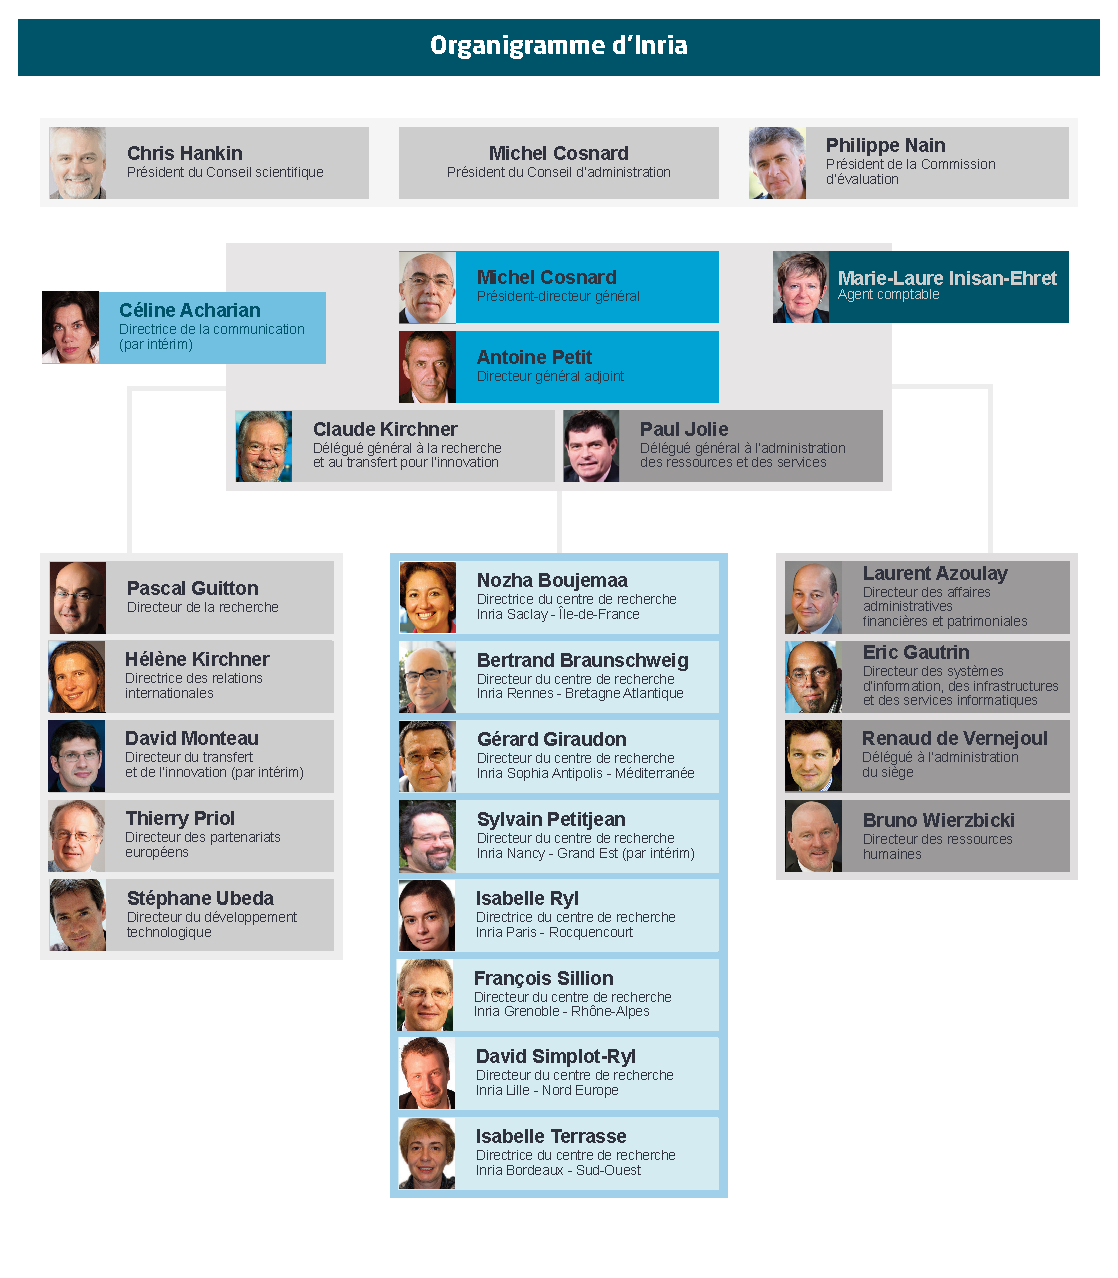
\includegraphics[scale=0.85]{data/organigrammeinria.pdf}
    \caption{Organigramme des différents services de l'INRIA\label{orga}}
    \end{figure}

    %% structure logique
    %% datas sur le pognon et les employés
  \section{Le service}
  Cette section présente le laboratoire PPS. Ce n'est pas à proprement parler
  un service de l'INRIA, car c'est un groupe de recherche multidisciplinaire
  regroupant des chercheurs de divers horizons, et de plusieurs structures de
  recherche.
    \subsection{Le laboratoire Preuves, Programmes  et Systèmes}
    PPS est un laboratoire qui regroupe les chercheurs venant de l'informatique
    et de la logique mathématique autour de l'idée que la logique et d'autres
    champs des mathématiques peuvent permettre d'élucider le sens de programmes,
    d'améliorer leur sûreté et réciproquement, que l'informatique est une source
    permettant aux mathématiques d'avancer.

    La majorité de la recherche menée par PPS gravite autour la correspondance
    de Curry-Howard: l'équivalence entre preuve et programmes, transformant
    le \lc\footnote{Le \lc{} est un formalisme mathématique
    qui constitue les fondements des langages de programmations du paradigme fonctionnels} en un
    outil utilisé pour établir des preuves mathématiques. Réciproquement, le
    savoir de la logique mathématique devient un élément de réponse pour les
    problèmes posés par l'industrie dans le domaine de l'informatique.

    \subsection{Thématiques de recherche du laboratoire}
      Les thématiques du laboratoire peuvent être regroupées en six directions
      principales :
      \begin{itemize}
        \item \textbf{Jeux et modèles de la programmation} : \\
          Les modèles de jeux permettent de modéliser mathématiquement
          l'interaction d'un programme avec son environnement. Ce champ de
          recherche débouche aujourd'hui sur des outils d'analyse et de
          certification des programmes
        \item \textbf{Théorie de la démonstration et \lc} :
          Ce domaine d'étude se concentre sur le développement de l'assistant
          de preuve Coq et les champs de recherche qui lui sont associés,
          tels que le calcul des constructions inductives.
        \item \textbf{Spécifications et réalisabilité} :
          L'objectif est, à partir d'un théorème mathématique, de trouver
          le programme équivalent. L'approche particulière de ce domaine est
          qu'au lieu de supposer une formule avant la preuve, la théorie de la
          réalisabilité considère les formules comme faisant partie des
          spécifications d'un programme.
        \item \textbf{Réécriture} :
          La théorie de la réécriture combine des éléments de la logique, de
          l'algèbre, du \lc, etc $\ldots$, et a pour but de transformer des
          programmes (et plus précisément des objets syntaxiques) à travers
          l'application de règle bien déterminées. Cette théorie propose
          un formalisme permettant de modéliser à la fois des langages
          fonctionnels, impératifs ou encore orientés objet.
          Les applications d'une telle théorie sont très diverses: la plus
          connue étant probablement l'optimisation d'un programme par le
          compilateur par le moyen de la réécriture de code.
          La théorie de la réécriture permet de formaliser et de prouver ces
          mécanismes.
        \item \textbf{Programmation} : \\
          Le laboratoire développe de nouvelles méthodes de programmations
          appliquées à de nombreux domaines qui vont des protocoles réseaux
          jusqu'au web. Ces développements sont étroitement liés à la
          logique mathématique, et permettent de mettre en évidence des
          propriétés sur ces programmes\footnote{Par exemple, le framework de
          développement web Ocsigen, donne la garantie de générer des pages
          web valides selon les standards W3C}.
        \item \textbf{Logique, Concurrence et Modélisation} : \\
          Un nouveau front de recherche s'est récemment ouvert à PPS, autour
          de la modélisation de la programmation dite concurrente (calculs de
          processus) et mobile, qu'il s'agisse d'en rechercher les fondements
          logiques, ou de les appliquer à une troisième science : la
          biologie, et plus précisément à la modélisation des processus de
          la biologie moléculaire.
      \end{itemize}

      \subsection{L'équipe \pir}
      L'équipe \pir{} est composée de chercheurs faisant partie du laboratoire
      PPS, mais également de scientifiques appartenant à l'université
      Paris-Diderot ou l'INRIA.

      Ses sujets de recherche sont les suivants :
      \begin{itemize}
        \item La recherche fondamentale autour de la correspondance entre preuve et programmes
        \item La recherche théorique autour du formalisme qui sous-tend les
          mécanismes de l'assistant de preuves Coq
        \item Un domaine d'implémentation: Coq, notamment en le considérant comme
          un langage de programmation avec des types-dépendants.
      \end{itemize}
      L'équipe développe notamment deux logiciels, Coq (présenté ci-après),
      et Pangolin, qui lui permet la certification de programmes fonctionnels.
      \subsubsection{L'assistant de preuves Coq}
      Le logiciel Coq est un outil de développement semi-interactif de
      preuves bâti autour d'un langage de programmation fonctionnelle
      fortement typé. Développé conjointement par plusieurs équipes INRIA et
      hors INRIA, Coq est utilisé tant pour la formalisation des
      mathématiques que pour la certification de propriétés de programmes.
      Naturellement doté de types dépendants, Coq a une carte à jouer comme
      langage de programmation à type riches. Un des objectifs de \pir dans
      ce cadre est le développement de bibliothèques de programmation
      certifiée, la certification du processus d'extraction de programme Coq
      vers des langages fonctionnels comme Objective Caml, ainsi que le
      développement de nouvelles méthodes de preuves pour Coq.

      Les principaux champs d'applications de Coq sont les suivants :
      \begin{itemize}
        \item L'écriture de programmes certifiés : les systèmes critiques
          (les transports, l'énergie, la santé, les télécommunications, la
          cryptologie, etc $\ldots$) ont besoin d'être rigoureusement conforme
          à leur spécification, pour pouvoir éviter tout disfonctionnement
          du logiciel. La preuve de programme consiste à s'assurer
          mathématiquement que le comportement d'un programme est conforme à
          ce qui est attendu, et Coq facilite ce travail de preuve de programme.
      \item La validation de preuves mathématiques : les publications
          scientifiques dans le domaine des mathématiques incluent parfois
          des preuves de plusieurs centaines de pages. Coq est un outil
          permettant de valider les preuves ainsi publiées. On peut citer
          le théorème de Fermat-Wiles ou encore Feit-Thompson comme exemples
          de cette application.
        \item Dans la recherche fondamentale en Informatique: c'est un outil
          qui permet de formaliser (et valider) la sémantique des langages de
          programmation et, qui est utilisé plus largement dans la théorie
          des langages de programmation.
      \end{itemize}

      \section{Le positionnement du stage dans les travaux de l'entreprise}
      L'utilisation d'un logiciel de documentation est très importante lors du
      développement d'un projet.
      Au sein du développement de Coq, Coqdoc possède plusieurs cas
      d'utilisations qui en font un outil très utilisé, et dont l'amélioration
      est supposée offrir plusieurs avantage. La liste suivante
      présente les différents cas d'utilisations de Coqdoc dans le projet :
      \begin{itemize}
        \item \textbf{Documentation de développement du compilateur :} \\
          Bien qu'une importante partie de Coq soit écrit en Caml, l'ensemble
          des bibliothèques standards, c'est à dire les outils pour Coq
          fournis avec le compilateur, sont écrites en Coq. Coqdoc permet donc
          de décrire le fonctionnement d'une importante partie du code source
          du compilateur.
        \item \textbf{Documentation utilisateur :} \\
          Une importante partie de la documentation explique le fonctionnement
          du projet Coq à l'utilisateur. Dans une documentation utilisateur,
          le code sert d'exemple aux explication fournies par la documentation.
        \item \textbf{Écriture de documents :} \\
          Cette application se distingue de l'écriture de documentation car
          elle n'est pas directement associée à un code source. L'objectif ici
          est d'inclure les avantages de Coqdoc (coloration syntaxique,
          mise en forme du code) dans des documents qui ne sont pas directement
          liés au compilateur, tels que des articles scientifiques ou des
          livres.
      \end{itemize}

      Coqdoc possède donc une grande importance au sein du projet Coq. La
      reconception de ce logiciel doit permettre d'offrir des fonctionnalités
      qui impacteront l'ensemble de ses utilisateurs.

\chapter{Travail effectué}
Cette section détaille le travail effectué au cours de ce stage de fin de tronc
commun. Nous détaillons tout d'abord les objectifs à atteindre en présentant
les outils utilisés, et en expliquant les spécificités propre à ce stage.
Nous expliquons ensuite les différentes phases de la conception du logiciel,
et les phases du développement. Enfin, nos offrons une analyse critique des
résultats que nous avons obtenus à l'issue de ce stage de fin de tronc commun.
%% 40 -> 50
  \section{Le cahier des charges}
  Cette section détaille les objectifs du stage à travers une analyse des outils
  existants (plus précisément, "l'ancien" Coqdoc, et Coq-tex),
  et nous détaillons les objectif à atteindre pour le nouveau Coqdoc.
    \subsection{Logiciels de documentation}
    Lors du développement d'un logiciel, le code source est souvent insuffisant
    pour détailler le fonctionnement du programme, car il manque en clarté et
    n'est pas toujours assez explicite.
    Le rôle de la documentation est de décrire les différents aspects du
    fonctionnement attendu du code source. Cette documentation est incluse
    dans les fichiers sources sous forme de commentaires, de façon à ce
    qu'elle soit facilement accessible aux développeurs.

    Le rôle d'un logiciel de documentation est d'extraire ces informations
    contenues dans le code source afin d'en constituer un guide de référence
    ou un manuel, sous forme de pages web ou de documents PDF.
    Cela permet au programmeur de bénéficier d'un document décrivant clairement
    le projet, et qui détaille les fonctionnalités accessibles au programmeur.

    L'utilisation d'un générateur de documentation possède plusieurs intérêts :
    \begin{itemize}
      \item \textbf{Facilité de mise à jour de la documentation :} \\
        Parce que la documentation est située dans le code source, lorsqu'un
        développeur modifie un fichier, il peut facilement mettre à jour cette
        documentation. Ainsi, le manuel de référence associé au code source
        évolue en même temps que celui-ci.
      \item \textbf{Mise en forme automatique de documents :} \\
        Les logiciels de documentation possèdent des règles de mise en forme
        des commentaires dans les documents produits. Ainsi, un générateur
        de documentation sait traiter les informations de mise en forme
        données par le programmeur, pour avoir une meilleure explication du
        code source (découpages logiques, titres, mettre en gras les éléments
        importants dans les commentaires).
      \item \textbf{Variété des formats de sortie :} \\
        Enfin, l'un des éléments les plus important est le fait qu'un logiciel
        de documentation sait gérer plusieurs formats de sorties pour la
        documentation, allant de la génération de pages web à la génération de
        PDF.
    \end{itemize}

    Les exemples \cref{source1,fig1} présentent un morceau de code documenté, et le rendu
    généré par coqdoc.
    \begin{figure}
      \lstinputlisting
        {data/source1.v}
        \caption{Exemple de fichier d'entrée donné à Coqdoc\label{source1}}
    \end{figure}

    \begin{figure}

      \fbox{
      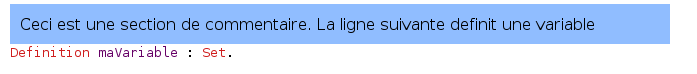
\includegraphics[trim=0mm 0mm 2cm 0cm,clip=true, width=\textwidth]{data/rendu1.png}}
      \caption{Exemple de rendu généré par Coqdoc à partir de la \cref{source1}}
      \label{fig1}
    \end{figure}

    \clearpage

    \subsection{Analyse de l'existant : Coqdoc}
    Le projet Coq avait déjà un logiciel de documentation de son code source.
    Cette section détaille les particularités de ce logiciel. L'un des objectifs
    du stage était d'avoir un nouveau Coqdoc dont le comportement est le plus
    proche possible de l'ancien : il doit pouvoir gérer les mêmes options et
    un rendu similaire. Cela permet de :
    \begin{itemize}
      \item Faciliter l'intégration du nouveau logiciel grâce à la
        rétro-compatibilité
      \item Avoir un rendu similaire par rapport aux pages de documentations
        générées auparavant
      \item Se servir de l'ancien logiciel comme référence pour un ensemble
        de tests fonctionnels et techniques
    \end{itemize}

    \subsubsection{Format des fichiers d'entrée}
    Comme beaucoup de logiciels de documentation, Coqdoc propose un langage de
    mise en forme de la documentation : ce sont des balises, qui, en étant
    présentes dans le code source, permettent de mettre en forme le fichier de sortie,
    et qui permettent de donner de plus amples informations à propos du code
    documenté.
    \begin{itemize}
      \item[] \textbf{Format des lignes de documentation :} \\
      Comme nous l'avons déjà vu, Coqdoc fait une distinction entre commentaires
      et documentation. En Coq, les commentaires sont préfixés par "(*" et se
      terminent par "*)". Coqdoc considère que tout commentaire commençant par
      "(**" est une portion de texte devant apparaître dans la documentation
      générée.
      \item[] \textbf{Titres :} \\
      Pour introduire des titres dans le document de sortie, l'utilisateur
      peut préfixer le début d'une ligne par 1 à 4 astérisques suivies d'une
      espace. Le nombre d'astérisques déterminant le niveau d'importance du
      titre.
      \item[] \textbf{Listes :} \\
        Toute ligne commençant par un tiret et précédée de \texttt{n} espaces
        est un élément d'une liste, dont le niveau de profondeur est déterminé
        par le nombre d'espaces
      \item[] \textbf{Séparateur horizontal :} \\
        Une ligne constituée uniquement de 4 tirets ou plus produit un
        séparateur horizontal
      \item[] \textbf{Emphase :} \\
        Il est possible de mettre en valeur des mots en les encadrant
        de tirets bas ("\texttt{\_}").
      \item[] \textbf{Verbatim :} \\
        On peut inclure du code dans de la documentation en encadrant cette
        portion de code de double chevrons (\texttt{<<} et \texttt{>>})
      \item[] \textbf{Cacher des portions de code :} \\
        A des fins de clarté dans la documentation, on peut cacher
        (ou afficher) des portions de code avec les délimitant avec
        \texttt{(* begin hide *)} et \texttt{(* end hide *)}
        (pour forcer l'affichage, il suffit de remplacer \texttt{hide} par \texttt{show})
      \item[] \textbf{Règles de traduction :} \\
        L'utilisateur peut définir des règles de traduction avec le mot clef
        printing, avec les délimiteurs suivants
        \begin{itemize}
          \item \texttt{\#} pour une sortie HTML
          \item \texttt{\%} pour une sortie en LaTeX
          \item \texttt{\$} pour une notation mathématique en sortie LaTeX
        \end{itemize}
    \end{itemize}
    Le listing \ref{source2} donne un exemple de ces règles de mise en forme
    dans le fichier d'entrée
    \lstinputlisting[label=source2,caption=Exemple des règles de mise en forme de Coqdoc]{data/source2.v}

    \subsubsection{Format des fichiers de sortie :}
    Le rôle de Coqdoc est d'effectuer une traduction du format d'entrée
    précédemment présenté vers plusieurs formats de sortie. Au cours
    de cette traduction, Coqdoc prends en compte les règles de mise en forme
    données en entrée pour la documentation et fait une analyse syntaxique du
    code source.

    La liste suivante détaille les différentes caractéristiques de Coqdoc dans
    la génération des fichiers de sortie

    \begin{itemize}
      \item \textbf{Mise en forme de la documentation} \\
        La première étape est la traduction des informations de mise en forme
        contenues dans la documentation. Le rôle de Coqdoc ici est de générer
        les balises adéquates dans le format de sortie
      \item \textbf{Analyse syntaxique du code source} \\
        Coqdoc a également pour rôle de mettre en forme le code source des
        fichiers lus en entrée. Pour cela il effectue une analyse syntaxique
        des sections de code source, et met en forme ces éléments de code
        source dans le fichier de sortie, en effectuant :
        \begin{enumerate}
          \item Une coloration syntaxique du code
          \item Le \textit{pretty print} de certains symboles selon les règles
            de traduction par défaut, et également selon celles définies
            par l'utilisateur. Par exemple, l'ancien coqdoc traduit
            automatiquement le symbole \texttt{->} en \texttt{$\rightarrow$}.
            Le tableau \cref{trad.coqdoc} donne une liste exhaustive des
            symboles traduits par coqdoc.
        \end{enumerate}
      \item \textbf{Gestion de la structure logique de la documentation} \\
        Coqdoc doit également gérer les règles de génération des fichiers selon
        la volonté de l'utilisateur. Ceci est fait avec des options passées à
        Coqdoc, qui permettent de définir si un seul fichier doit être généré
        (pour un manuel de référence par exemple) ou plusieurs
        (pour une documentation utilisateur). Il y a également des règles par
        défaut selon le format de fichier de sortie : par exemple, pour une
        sortie HTML, plusieurs fichiers seront générés, tandis qu'une sortie
        en LaTeX entraînera la génération d'un seul fichier mettant en commun
        tous les fichiers d'entrée.
      \item \textbf{Génération des liens hypertextes} \\
        Une autre partie du travail de Coq est la génération des liens
        hypertextes, qui permettent de faire référence à :
        \begin{enumerate}
          \item Des \textbf{identifiants déclarés dans d'autres fichiers} : en
            effet,
            l'utilisateur fournit souvent plusieurs fichiers à documenter, et
            un identifiant peut avoir une importance dans plusieurs fichiers.
            Cette génération de liens permet de faciliter la lecture de la
            documentation, en proposant un lien vers la déclaration de
            l'identifiant, pour permettre à l'utilisateur d'obtenir de plus
            amples informations à propos de celui-ci si nécessaire.

            Cette génération de liens se base sur des fichiers issus de la
            compilation ayant pour extension \texttt{.glob} qui détaille les
            identifiants déclarés dans un fichier. Grâce à ceux ci, Coqdoc peut
            ainsi générer des références entre plusieurs fichiers.
          \item Coqdoc propose également de générer des \textbf{références à
            la documentation de la bibliothèque standard}; cela permet de
            fournir à l'utilisateur un moyen rapide de s'informer sur un
            élément faisant partie du langage Coq.
          \item De la même manière, il est possible de faire \textbf{référence
            à une bibliothèque externe}, pour pouvoir détailler de celle-ci
            avec le projet documenté.
        \end{enumerate}
    \end{itemize}

    \subsubsection{Nécessités d'amélioration}
    Nous détaillons dans cette section les raisons qui motivent la refonte
    du logiciel Coqdoc :
    \begin{itemize}
      \item \textbf{Conception du logiciel} : \\
        La conception de Coqdoc rend difficile son maintien. C'est un logiciel
        qui manque de structure logique et dont la conception souffre de
        plusieurs défauts. Une refonte permettrait d'avoir une structure
        logique plus cohérente, et faciliterait le maintien d'un tel outil.
      \item \textbf{Extensibilité} : \\
        Coqdoc possède un manque important d'extensibilité. Un tel outil
        bénéficierait d'une plus grande variété de cas d'utilisation qui
        gravitent autour du même concept de présentation de code et de mise
        en forme d'une documentation autour. On peut par exemple citer
        la génération d'une documentation interactive, où l'on peut rejouer
        les preuves Coq dans le navigateur internet.
      \item \textbf{Redondance de certains éléments logiciels} : \\
        Coqdoc fait une analyse de code source, et celle-ci est faite par de
        nombreux outils dans la suite logicielle de Coq (le compilateur,
        l'éditeur CoqIDE, Coq-tex). La redondance de ces éléments peut être
        retirée en réécrivant Coqdoc, et en proposant une interface unifiée.
    \end{itemize}

    \subsection{Analyse de l'existant : Coq-tex}
    Un des autres objectifs de ce stage était d'offrir un remplacement pour
    Coq-tex, un des autres outils du projet Coq. Nous détaillons dans une
    première partie l'approche qu'offre Coq-tex à propos de la programmation,
    pour ensuite détailler son fonctionnement.

    \subsubsection{Programmation lettrée}
    La programmation lettrée (\textit{literate programming}) est une approche
    de la programmation introduite par \textbf{Donald Knuth} dans laquelle
    le code source du programme suit le flux de pensée de l'auteur : à la
    manière d'un article, le programmeur introduit les concepts de son
    programme dans l'ordre logique de la pensée humaine, au lieu de suivre
    l'ordre logique et la manière demandée par le compilateur. A travers un
    ensemble de fonctions (ou plutôt de macros), l'auteur peut cacher
    l'abstraction demandée par l'ordinateur pour s'exprimer dans un langage
    plus proche du langage naturel.

    Ainsi les outils pour la programmation lettrée permettent de générer deux
    versions d'un code source : une nouvelle version du code adaptée à la
    génération d'un \textbf{programme} par un compilateur, et une autre version
    qui elle est sous la forme d'une \textbf{documentation} à destination d'un
    lecteur.

    Cette approche est particulièrement intéressante pour expliquer des
    programmes Coq car elle permet de changer l'ordre logique des différents
    éléments du programme pour ainsi avoir une version plus facile à comprendre
    pour des humains : la preuve de théorèmes mathématiques en Coq peut ainsi
    être plus facile à comprendre pour un lecteur, et à partir du programme
    fournissant la preuve, il est possible d'obtenir un article scientifique
    expliquant cette preuve.

    \subsubsection{Fonctionnement de Coq-tex}
    Coq-tex est un outil se rapprochant de ce concept de programmation lettrée.
    Le programme prend en argument un fichier LaTex, et extrait les phrases
    Coq contenues dans celui-ci, pour y insérer à la place le résultat de
    leur interprétation.

    La production d'un document LaTeX bénéficie ainsi d'une phase
    d'interprétation du code Coq contenu dans ce document, pour pouvoir fournir
    le résultat de l'interprétation de code avec une version récente de
    l'interprète Coq. Cet outil est notamment utilisé pour générer la documentation
    officielle du projet Coq.

    Le fonctionnement de Coq-Tex gravite autour de 3 environnements \footnote{Un
    environnement en LaTeX est une portion de code entourée des balises
    \texttt{$\backslash$begin\{environnement\}} et
    \texttt{$\backslash$end\{environnement\}}, où \texttt{environnement} est
    le nom de l'environnement. Le texte contenu dans ces balises sera ainsi
    traité selon le type d'environnement dans lequel il est inclut.}
    insérés
    dans un fichier LaTeX. La liste suivante détaille le comportement de
    chacun :
    \begin{itemize}
      \item \texttt{coq\_example} : \\
        Le code contenu dans ces balises sera extrait et évalué par
        l'interprète phrase par phrase. Chacune de ces phrases sera copiée
        dans le fichier de sortie, et sera suivie du résultat de son
        interprétation.
      \item \texttt{coq\_example*} : \\
        Le code contenu dans ces balises sera extrait et interprété, et il
        sera recopié dans le fichier de sortie. Cependant, les réponses de
        l'interprète seront ignorées.
      \item \texttt{coq\_eval} : \\
        Les phrases contenues dans l'environnement \texttt{coq\_eval} seront
        évaluées silencieusement. Seulement le résultat de leur évaluation sera
        inclut dans le document de sortie.
    \end{itemize}

    \subsubsection{Facilité de fusion avec Coqdoc}
    Coq-tex reprend la même idée que Coqdoc dans le sens où ces deux outils
    ont un rôle de traduction : ils prennent un document d'entrée pour effectuer
    une évaluation de certaines portions du code contenues dans celui-ci, afin
    de générer un document mis en forme.

    Ainsi ces deux outils ont des rôles de documentation du code source, et
    partagent d'importantes similarités dans leur fonctionnement. Une fusion
    de ces deux outils apparaît donc comme logique puisqu'elle facilitera
    ainsi la maintenance de l'outil, et regroupera des sections logique qui
    auparavant étaient dupliquées dans deux programmes.

    Intégrer cet outil dans Coqdoc permet également d'enrichir Coq-tex, en
    permettant à l'utilisateur de profiter de la diversité des formats de
    sortie de Coqdoc et en rajoutant les caractéristique de l'outil Coq.

    \clearpage
    \subsection{But général : refonte de Coqdoc}
    Les sections précédentes on démontré le besoin de réécrire le logiciel
    Coqdoc. La majeure partie de mon stage s'est concentrée sur la conception
    et la réécriture de ce logiciel.

    Nous rappelons brièvement les objectifs introduit dans les sections
    précédentes concernant le logiciel produit pendant ce stage :
    \begin{itemize}
      \item Le nouveau Coqdoc doit avoir un comportement le plus proche
        possible de l'ancien Coqdoc.
      \item Il doit également remplacer Coq-tex, l'outil de programmation
        lettrée.
      \item L'attention doit être portée sur une architecture extensible, qui
        permette aux développeurs de rajouter de nouveaux comportements
        et d'enrichir le logiciel. \\
    \end{itemize}

    En arrivant dans ce stage, j'avais également plusieurs objectifs personnels
    que je désirais réaliser dans ce stage.

    Tout d'abord, améliorer
    mes compétences dans le langage de programmation OCaml (une présentation
    du langage est incluse ci-après), qui est un langage dont les spécificités
    m'intéressent beaucoup.

    Une autre aspect était de découvrir les sujets de recherches au sein de
    l'équipe \pir, et de voir si les sujets explorés m'intéressaient.

    Enfin, le sujet de ce stage me permet également de valider les acquis de
    ma formation à travers la conception et l'écriture d'un logiciel complexe.

  \section{Compte-rendu d'activité}
  Nous détaillons dans cette section les différents aspects du développement
  de Coqdoc au cours de ce stage.  Nous introduisons tout d'abord les outils
  utilisés, puis nous détaillons la phase de conception du logiciel, tout
  d'abord l'architecture générale puis les choix techniques de cette
  conception. Enfin, nous détaillons chaque étape du développement de Coqdoc
  au cours du stage.
    \subsection{Présentation des outils utilisés}
    Le choix du langage s'est naturellement porté sur OCaml pour le
    développement de Coqdoc, et cela pour plusieurs raisons. La liste
    suivante détaille les différents avantages à utiliser OCaml :
    \begin{itemize}
      \item \textbf{Langage du compilateur Coq} : \\
        Coq est principalement codé en OCaml. Coq et OCaml sont des langages
        de programmations partageant d'important traits communs : ils sont tout
        deux du paradigme fonctionnel et sont statiquement typés. L'utilisation
        d'OCaml permet d'apporter des garanties sur la validité du compilateur
        Coq, et le fait que les deux langages soient proche facilite le
        développement de Coq.
      \item \textbf{Écriture de compilateurs} : \\
        OCaml est particulièrement adapté pour l'écriture de compilateurs.
        Coqdoc peut être considéré comme un compilateur car il passe un fichier
        en représentation abstraite, procède à une évaluation et génère un
        document prêt à être utilisé. Le typage fort de OCaml, le haut niveau
        d'abstraction et l'aspect fonctionnel du langage facilite grandement
        l'écriture de compilateurs.
      \item \textbf{Limitation des dépendances, et facilité d'intégration} : \\
        Une raison plus pragmatique est également que pour faciliter la gestion
        du projet, rajouter des dépendances à d'autres logiciels (par exemple,
        d'autres compilateurs de langage) n'est pas une bonne chose, tant pour
        la portabilité que l'évolution de la suite d'outils Coq. Choisir
        OCaml et les outils qui lui sont liés facilitent le processus
        d'intégration de Coqdoc au sein de Coq
    \end{itemize}
    %% FIXME ?
    \subsection{Conception de l'architecture du logiciel}
    Coqdoc se doit d'être extensible. Pour cette raison, nous avons dû apporter
    une attention particulière sur ce point lors de la conception de
    l'architecture logicielle.
    Le diagramme \cref{fig.devchain} montre l'architecture simplifiée de Coqdoc.

    Nous résumons les différentes étapes d'une compilation effectuée par
    Coqdoc :
    \begin{enumerate}
      \item Lecture d'un ou plusieurs fichiers d'entrée
      \item A partir de ces fichiers une analyse syntaxique est effectuée.
        Ils sont alors représentés de manière abstraite, ceci afin de
        s'affranchir de la structure linéaire des fichiers d'entrée, et de
        faciliter les différentes phases de traitement.
      \item La phase d'évaluation permet d'obtenir la représentation finale
        des fichiers d'entrée : les commandes entrées dans Coqdoc (l'ajout
        de symboles par exemple) sont évaluées, tandis que le code sera annoté
        et mis en forme.
      \item Un des choix suivant est de sauvegarder cette représentation
        finale sous forme de Vdoc : c'est un format de fichier qui détaille
        la représentation abstraite des documents traités.
        Un fichier Vdoc peut ainsi être relu par Coqdoc pour générer plusieurs
        types de documentation, sans avoir à réévaluer le fichier. Cela facilite
        la portabilité des documents, tout en permettant à l'utilisateur de faire
        des ajustements plus fins concernant la documentation générée (puisque
        l'on se situe après l'évaluation, le code est par exemple déjà annoté
        pour permettre la coloration syntaxique)
      \item L'autre choix est de générer un ou plusieurs documents finaux.
        On utilise pour cela un module d'impression, qui est en mesure de
        générer différents types de documentation.
        Ce module d'impression est paramétré par des "spécifications", qui
        détaillent le format de sortie des documents finaux. En effet, le
        module d'impression attend un ensemble de fonctions qui lui
        permettent de générer un document final.
        Il est ainsi facilement extensible, car pour rajouter un format de
        sortie, il suffit de donner sa spécification au module d'impression.
    \end{enumerate}

    Les sections suivantes détaillent chacune des étapes de la compilation
    d'un document par Coqdoc.
    %% FIXME: détailler les sous modules d'impression sur le graphe
    \begin{figure}
      \fbox{\includegraphics[scale=0.5]{data/devchain.png}}
      \caption{Représentation de la chaîne de compilation de Coqdoc}
      \label{fig.devchain}
    \end{figure}
    %% traitement
    \clearpage
    \subsection{Traitement du langage d'entrée}
    Cette section détaille les différentes phases d'analyse pour traiter le
    langage d'entrée de Coqdoc. Nous expliquons tout d'abord les méthodes
    pour effectuer une analyse syntaxique, puis nous détaillons chaque phase
    de traitement du langage.
    Pour expliquer plus facilement le traitement du langage d'entrée, nous
    prenons un exemple fil rouge qui accompagnera notre explication de la
    chaîne de traitement. Le listing \ref{finput} montre le fichier d'entrée
    donné à Coqdoc.
    \lstinputlisting[float,label=finput,caption=Fichier d'exemple Coq]{data/finput.v}

    \subsubsection{Traitement du langage}
    \label{trait}
    Le traitement d'un langage se fait en plusieurs phases logiques. Nous
    rappelons brièvement celles-ci :
    \begin{itemize}
    \item[] \textbf{Analyse lexicale}  :\\
      La première étape est l'analyse lexicale. Cette phase vise à décomposer
      le document d'entrée en entités logiques, facilitant le traitement
      des données par la suite.
    \item[] \textbf{Analyse syntaxique} :\\
      La deuxième étape du traitement d'un langage est l'analyse syntaxique.
      Celle-ci vise à fournir une représentation de plus haut niveau pour
      la suite de la chaîne de traitement. L'analyseur lexical génère un
      ensemble d'entités, que l'analyseur syntaxique regroupera en structures
      de données plus riches.
      \item[] \textbf{Arbre de syntaxe concrète} :\\
      L'analyse syntaxique donne souvent lieu à la génération d'un arbre
      de syntaxe concrète. Cet arbre est une représentation intermédiaire
      entre le document d'entrée et l'arbre de syntaxe abstraite, qui
      lui représente la structure de donnée sur laquelle les traitements sont
      appliqués. La différence principale entre ces deux types d'arbres est
      qu'un arbre de syntaxe concrète est beaucoup plus proche du document
      source, est a une structure de moins haut niveau (plus proche du
      document source) que l'AST.  Cela permet ainsi d'effectuer la
      transformation inverse, pour revenir à un document très proche du
      document source.
      \item[] \textbf{Arbre de syntaxe abstraite} :\\
      L'arbre de syntaxe abstraite est la représentation choisie pour appliquer
      des traitements sur le document d'entrée. Le haut niveau d'abstraction
      de cette structure de donnée permet de facilement modifier ses différent
      éléments, ceci afin de pouvoir effectuer une traduction simple vers la
      représentation finale, et générer le document de sortie.
    \end{itemize}
    \subsubsection{Découpage logique du document}
    La première phase de traitement du document est un découpage logique
    en phrases de différents types : la documentation, le code et les
    commentaires.
    Ceci est fait selon les délimiteurs respectifs de la documentation et
    des commentaires. Tout ce qui n'est pas contenu entre ces délimiteurs
    est considéré comme du code.

    Chaque élément de code est ensuite découpé en phrases.
    Ce découpage est
    fait selon le fait que chaque phrase Coq se termine par un point. Cela
    permet de simplifier le traitement sur chaque instruction du fichier d'entrée.
    A la fin de cette phase de traitement, nous avons donc un ensemble
    de phrases, chacune appartenant à l'un des types suivants
    \begin{itemize}
      \item \textbf{De la Documentation} sous forme de chaînes de caractères
      \item \textbf{Des commentaires} sous forme de chaînes de caractères
      \item \textbf{Du code} sous forme de chaînes de caractères, chacune
        de ces chaînes étant terminées par un point.
    \end{itemize}

    L'exemple \cref{ast1} illustre la représentation de notre fichier après
    cette première phase de traitement. Chaque noeud représente un élément
    logique de notre documentation, le contenu de ce noeud étant les chaînes
    de caractères stockées dans le noeud de l'arbre de syntaxe abstrait.
    \begin{figure}
      \fbox{
      \includegraphics[scale=0.5]{data/ast1.png}}
      \caption{Première représentation abstraite}
      \label{ast1}
    \end{figure}
    \clearpage
    \subsubsection{Analyse de la documentation}
    La deuxième étape consiste ensuite au traitement de la documentation.
    Chaque élément du type documentation est donc analysé une seconde fois,
    ceci afin d'effectuer une séparation des différents éléments logiques
    de la documentation. Après l'analyse, cette documentation est représentée
    sous la forme d'un arbre qui représente la structure hiérarchique des
    éléments de mise en forme.

    La liste suivante détaille différents types de noeud dans notre
    documentation :
    \begin{itemize}
      \item \textbf{Éléments finaux} : (contiennent des chaînes de caractère ou rien)
        \begin{itemize}
            \item Titre
            \item Règle horizontale
            \item Notation : notations spéciales pour dépendant du format de sortie
            \item Code Verbatim : code à imprimer dans la documentation
            \item Contenu : représente les chaînes de caractère simples
        \end{itemize}
      \item \textbf{Éléments récursifs} : (contiennent des éléments de documentation)
        \begin{itemize}
          \item Listes : une liste contient soit d'autres listes, soit des
                éléments de documentation
          \item Emphase : l'emphase doit pouvoir mettre en valeur des éléments
                de la documentation (par exemple, des éléments d'une liste ou
                du code verbatim)
        \end{itemize}
      \item \textbf{Éléments à évaluer} : (seront supprimés après la phase d'évaluation)
        \begin{itemize}
          \item Ajout de règles de notation
          \item Suppression de règles de notation
          \item Commandes : Un ajout du nouveau Coqdoc est la gestion de
                commandes plus poussées dans le fichier d'entrée. Celles-ci
                seront remplacés par des noeuds de documentation après la
                phase d'évaluation
        \end{itemize}
    \end{itemize}
    Après application de la transformation, la documentation est transformée
    d'une chaîne de caractères à une hiérarchie d'éléments décrivant le contenu.
    La \cref{ast2} détaille par exemple la hiérarchie obtenue pour la
   documentation après traitement de celle-ci
    \begin{figure}
      \includegraphics[scale=0.45]{data/ast2.png}
      \caption{Traitement de la documentation}
      \label{ast2}
    \end{figure}

    \subsection{Interactions avec l'interprète}
    Pour pouvoir effectuer la mise en forme des différentes sections de code,
    deux approches étaient possibles :
      \begin{itemize}
        \item Effectuer une analyse lexicale et syntaxique du code, pour
          en obtenir les différents éléments logique, et coder un
          \textit{pretty-printer} pour imprimer le code de manière lisible.
          Cela impose de traiter un langage très complexe (composé d'un nombre
          important de mots clefs et de constructions syntaxiques), et de
          complexifier de manière importante le logiciel. Écrire un module
          d'analyse du langage Coq insère également de la redondance dans le
          projet, puisque le compilateur Coq effectue déjà cette analyse. Cette
          approche était celle de l'ancien Coqdoc.
        \item Réutiliser l'interprète pour nous donner des informations sur
          du code. A partir d'un protocole existant, nous envoyons des séquences
          de code, et l'interprète est en mesure de renvoyer une version imprimée
          de manière jolie, avec les bonnes annotations syntaxique.
          Parce que ce protocole fait l'interface entre l'interprète et d'autres
          logiciels, il est facilement extensible, car nous avons accès à tous
          les éléments du compilateur. La duplication de code est donc inexistante
          avec cette approche, et l'extension du protocole d'interaction entre
          l'interprète et les logiciels qui l'utilisent est bénéfique pour tous
          ces logiciels.
      \end{itemize}
    C'est la seconde approche qui a été choisie : elle permet de réutiliser
    l'existant tout en facilitant une extension de ces interactions à nos besoin

    \subsubsection{Protocole d'interaction}
    Le protocole d'interaction de l'interprète est une communication sous forme
    de XML, ce qui permet de l'utiliser avec une grande variété d'outils.
    La liste suivante présente les requêtes de ce protocole :
    \begin{itemize}
      \item \texttt{evars}, \texttt{goals}, \texttt{hints}, $\ldots$ : Commandes utilisées pour les preuves.
      Coqdoc n'en aura pas l'utilité.
    \item \texttt{inloadpath} : permet de savoir si un dossier est dans le chemin
      de chargement de Coq
    \item \texttt{interp} : Prends une phrase Coq sous forme de chaîne, et effectue
      l'interprétation de cette phrase.
    \item \texttt{rewind} : permet de revenir en arrière dans l'exécution
    \item \texttt{status} : donne des informations sur le status de l'interprète
      \item \texttt{quit} : ferme le protocole d'interaction
    \end{itemize}

    %% Presentation generale des besoin dans les assistants de preuves
    %% Detailler l'utilisation du protocole a l'existant
    %% Etendre ce protocole pour Coqdoc
    \subsection{Extension du protocole d'interaction}
    Avant de pouvoir être utilisé sous cette forme, le protocole d'interaction
    a besoin d'être étendu pour pouvoir annoter du code, et situer les
    différents identifiants.

    Deux commandes ont donc été développés afin de répondre aux besoins de Coqdoc
    \begin{itemize}
      \item \texttt{locate} : prends un identifiant sous forme de chaîne de caractères,
      et renvoie sa localisation (dans quel fichier, module, et sous module).
      Cette commande doit permettre de pouvoir, a partir d'informations obtenues
      sur le code, permettre de reconnaître les identifiant, et ainsi pouvoir
     générer des liens vers l'endroit où ils sont déclarés dans la documentation
     produite.
      \item \texttt{prettyprint} :
      Cette commande prends une chaîne de caractère, et renvoie une version
      structurée selon les différents éléments la composant : mots clefs,
      identifiants, nombres, etc $\ldots$. Elle doit de plus donner
      les informations de mise en forme du code (par exemple, l'indentation). \\
    \end{itemize}

    Tandis que le développement de la commande \texttt{locate} a été rapide,
    le développement de la commande prettyprint a été compliqué car il a fallu
    combler un manque du logiciel Coq.

    L'approche idéale pour effectuer l'annotation serait d'utiliser
    l'arbre de syntaxe concrète de Coq. Comme expliqué dans la \cref{trait},
    cet arbre de syntaxe doit théoriquement être en mesure de donner les bonnes
    annotations puisqu'il possède encore beaucoup d'informations d'ordre
    syntaxique. Son niveau d'abstraction est théoriquement adapté à nos besoins,
    car il représente encore fidèlement le code source que Coqdoc cherche à
    traiter. Cependant cet arbre de syntaxe concrète n'existe pas dans Coq,
    qui fait une traduction directement vers une représentation de haut niveau.

    L'approche la plus efficace aurait été de changer la chaîne de traitement
    de Coq pour pouvoir y insérer cet arbre de syntaxe concrète, mais cela
    impose une importante réflexion et beaucoup de changement de code. Au
    vu de la durée du projet, cette solution a été rejetée immédiatement car
    elle était trop complexe pour le temps disponible.

    Pour implémenter cette commande, il faut donc se reposer sur l'arbre de
    syntaxe abstraite, qui possède une représentation de très haut niveau,
    et dont l'annotation est complexe.

    %%% FIXME
    Un des mécanismes de traduction de l'arbre de syntaxe vers des chaînes de
    caractères est le \textit{pretty-printer} de Coqdoc. Son rôle est
    d'imprimer de manière correctement indentée l'arbre de syntaxe.
    Instrumenter le code du \textit{pretty-printer} à nos besoins nous
    permettrait ainsi de profiter de cette étape de traduction de l'arbre de
    syntaxe vers le texte. L'objectif est donc de modifier ce module de Coq
    pour, lors de la traduction, conserver les types de l'arbre, et ainsi
    pouvoir effectuer facilement une coloration syntaxique du coté de Coqdoc.

    La traduction du module d'impression de Coq se fait directement vers des
    chaînes de caractères. Ceci est problématique car cela enlève toutes les
    informations sémantiques qui serviraient à Coqdoc. La première approche
    que nous avons adopté était donc de modifier ce module d'impression, pour
    qu'au lieu de traduire vers des chaînes de caractères, il effectue une
    traduction vers un arbre de syntaxe allégé, chaque noeud ayant pour contenu
    les chaînes de caractère issues de l'impression.

    La première tentative de réécriture du module d'impression consistait
    en la transformation du code de façon à accueillir des types génériques.
    Cela permet d'avoir :
    \begin{itemize}
      \item L'ancien comportement du module d'impression, sans modifier le code
        l'utilisant
      \item Un nouveau comportement permettant la traduction vers la
        structure de donnée adaptée pour Coqdoc
    \end{itemize}

    Cette approche impose de redéfinir un ensemble conséquent de types :
    il faut reprendre les types de l'arbre de syntaxe abstraite pour créer
    une version de cet arbre avec des chaînes de caractère contenant le
    résultat de l'impression des noeuds. Il faut également réécrire une partie
    importante du module d'impression afin d'accueillir ces deux types (le type
    préexistant et celui que nous créons). La \cref{trad1} présente
    l'inclusion du module au sein de l'impression de Coq. Cet arbre annoté
    correspond à ce que l'on désire obtenir du coté Coqdoc. Cette structure
    contient toutes les informations nécessaires pour effectuer l'impression
    du code, tout en conservant la sémantique nécessaire pour effectuer des
    traitements dessus.

    Cette méthode de traduction ne fut pas terminée pour des raisons de temps.
    La phase de réécriture que j'ai entreprise était très coûteuse en temps,
    et nous n'avions pas les garanties qu'à l'issue de cette réécriture le
    résultat serait acceptable. En effet, même si cette réécriture avait put
    être achevée à temps, la mise en place de tests et la correction du module
    écrit aurait également pris beaucoup de temps. Face aux objectifs du stage
    et face aux impératifs de temps, nous avons donc adopté une méthode dont
    la qualité des résultats serait moindre, mais dont le développement et la
    validation seraient plus rapide.

    Cette deuxième approche instrumente toujours le code du module d'impression
    afin d'obtenir une version de l'arbre annotée. Cependant, plutôt que de
    procéder à une réécriture complète du type de l'arbre, nous modifions la
    phase d'impression de cet arbre. L'impression de l'arbre de syntaxe passe
    par un ensemble réduit de fonctions. En modifiant ces fonctions à nos
    besoin, nous pouvons ainsi, selon le contexte, sélectionner le mode
    d'impression. Soit l'impression par défaut est utilisée, soit, lors de
    l'interaction avec Coqdoc, nous utilisons le mode d'impression modifié.

    Comme décrit précédemment, l'interaction entre l'interprète et Coqdoc se
    fait au moyen d'un protocole XML. En réécrivant les fonctions d'impression,
    au lieu de générer la version par défaut du code, nous générons une version
    annotée par XML : chaque noeud appelant les fonctions d'impression est
    ainsi inclus dans des balises XML portant le type du noeud. La \cref{xml} schématise
    cette traduction. Le module d'impression peut ainsi générer au choix,
    selon la destination une version annotée ou pas du résultat de
    l'impression. L'implémentation et l'intégration d'une telle fonctionnalité
    fut rapide et facile à tester, et a posteriori, c'était le meilleur compromis
    entre le temps et la qualité de l'implémentation.
    \begin{figure}
  \begin{tikzpicture}
    %% Rectangle
    \draw (-5,-3) -- (-5,1);
    \draw (-5,-3) -- (2,-3);
    \draw (2,1) -- (-5,1);
    \draw (2,1) -- (2,-3);

    %% graphe1
    \node[text width=6cm] (titre1) at (0,1.5) {Arbre de syntaxe};
    \node[draw] (Noeud1) at (-1,0) {Noeud1};
    \node[draw] (Expression1) at (-3,-1) {Expresion1};
    \node[draw] (Element3) at (1,-1) {Element3};
    \node[draw] (Element1) at (-4,-2) {Element1};
    \node[draw] (Element2) at (-2,-2) {Element2};
    \draw[->] (Noeud1) -> (Expression1);
    \draw[->] (Noeud1) -> (Element3);
    \draw[->] (Expression1) -> (Element1);
    \draw[->] (Expression1) -> (Element2);

    % Rectangle 2
    \draw (3,-3) -- (3,1);
    \draw (3,-3) -- (10,-3);
    \draw (10,1) -- (3,1);
    \draw (10,1) -- (10,-3);

    % graphe2
    \node[text width=6cm] (titre2) at (8,1.5) {Arbre annoté};
    \node[draw] (INoeud1)      at (7,0) {"Noeud 1:"};
    \node[draw] (IExpression1) at (5.75,-1) {"( \_ + \_ )"};
    \node[draw] (IElement3)    at (8.5,-1) {"Element3"};
    \node[draw] (IElement1)    at (4.5,-2) {"Element1"};
    \node[draw] (IElement2)    at (7,-2) {"Element2"};
    \draw[->] (INoeud1) -> (IExpression1);
    \draw[->] (INoeud1) -> (IElement3);
    \draw[->] (IExpression1) -> (IElement1);
    \draw[->] (IExpression1) -> (IElement2);

    %%graph3
    \node[text width=6cm] (titre3) at (4,-4.25) {Sortie Texte};
    \node[draw] (Pp) at (3,-5) {"Noeud1: (Element1 + Element2): Element3"};

   \node[text width=6cm] (lab1) at (-2.6, -4) {Impression};
   \draw[->] (-4,-3) to [bend right] (-1.2,-5);
   \node[text width=6cm] (lab2) at (11.5, -4) {Impression};
   \draw[->] (8,-3) to [bend left] (7.1,-5);

   \node[text width=6cm] (lab3) at (5, 2) {Traduction};
   \draw[->,red] (1,1) to [bend left] (5,1);

   \draw[->, dashed] (8,-3) to (8, -6);
   \node[text width=6cm] (xml1) at (10,-6.5) {Protocole XML};
  \end{tikzpicture}
  \caption{Traduction de l'arbre de syntaxe abstraite\label{trad1}}
\end{figure}

    \begin{figure}
  \begin{tikzpicture}
    %% Rectangle
    \draw (-2,-3) -- (-2,1);
    \draw (-2,-3) -- (5,-3);
    \draw (5,1) -- (-2,1);
    \draw (5,1) -- (5,-3);

    %% graphe1
    \node[text width=6cm] (titre1) at (3,1.5) {Arbre de syntaxe};
    \node[draw] (Noeud1) at (3,0) {Noeud1};
    \node[draw] (Expression1) at (1,-1) {Expresion1};
    \node[draw] (Element3) at (4,-1) {Element3};
    \node[draw] (Element1) at (0,-2) {Element1};
    \node[draw] (Element2) at (2,-2) {Element2};
    \draw[->] (Noeud1) -> (Expression1);
    \draw[->] (Noeud1) -> (Element3);
    \draw[->] (Expression1) -> (Element1);
    \draw[->] (Expression1) -> (Element2);

    %%print par défaut
    \draw (-5.5,-5) -- (-0.5,-5);
    \draw (-5.5,-5) -- (-5.5,-7);
    \draw (-5.5,-7) -- (-0.5,-7);
    \draw(-0.5,-5) -- (-0.5,-7);

    \node[text width=6cm] (titre3) at (-1,-4.25) {Sortie Texte};
    \node[text width=6cm] (Pp) at (-2,-6) {"Noeud1: \\ (Element1 + Element2):\\     ~~~~Element3"};


    \draw (0.8,-5) -- (0.8,-9) -- (9,-9) -- (9,-5) -- (0.8,-5);
    \node[text width=6cm] (titre3) at (5,-4.25) {Sortie Annotée};
    \node[text width=8cm] (Pp) at (5,-7) {
    "$\textless$noeud1$\textgreater$Noeud1: \\
     ~~~~$\textless$expression1$\textgreater$ \\
     ~~~~~~~~($\textless$element1$\textgreater$Element1$\textless$/element1$\textgreater$ \\
     ~~~~~~~~ + $\textless$element2$\textgreater$Element2$\textless$/element2$\textgreater$) \\
     ~~~~$\textless$/expression1$\textgreater$:
     ~~~~$\textless$element3$\textgreater$Element3$\textless$/element3$\textgreater$ \\
     $\textless$/noeud1$\textgreater$"};

    \node[text width=6cm] (plop) at (-3,-3) {Impression};
    \draw[->] (-2,-2) to [bend right] (-5,-5);

    \draw[->, dashed] (-3,-7) -- (-3,-11);
    \node[text width=6cm] (stdout) at (-2,-12) {Sortie Standard};

    \node[text width=6cm] (plop1) at (10,-3) {Impression};
    \draw[->] (5,-2) to [bend left] (7,-5);

    \draw[->, dashed] (5,-9) -- (5,-11);
    \node[text width=6cm] (stdout) at (7,-12) {Protocole XML};

  \end{tikzpicture}
  \caption{Traduction vers une mise en forme XML\label{xml}}
\end{figure}

    \clearpage

    Du coté Coqdoc, il est facile de gérer ce type de messages à partir du XML.
    En effet, en effectuant une seconde passe sur le contenu du message, nous
    obtenons une hiérarchie que nous retraduisons dans une version adaptée à
    nos besoins. Cette nouvelle version comporte les types qui nous intéressent
    du point de vue Coqdoc, avec une sémantique du code très proche de nos
    objectifs.

    \subsection{Traitement du code annoté}
    Une fois la hiérarchie du code constituée, et son contenu correctement
    indenté par l'interprète de Coq, il est facile d'appliquer des traitements
    à ce code.

    Les traitements à effectuer sur une portion de code sont les suivants :
    \begin{itemize}
      \item \textbf{Coloration syntaxique} : \\
        Pour chaque type de noeud de l'arbre (correspondant à une expression),
        il faut décider à quel type de coloration il appartient (mot clef,
        identifiant, littéral, etc$\ldots$).
      \item \textbf{Règles de notations} : \\
        L'utilisateur peut définir des règles de traductions concernant
        certaines "phrases" de code, et Coqdoc doit les appliquer, plus celles
        déjà présentes par défaut.
      \item \textbf{Gestion des identifiants} : \\
        Coqdoc doit être capable de reconnaître les identifiants afin de pouvoir
        y appliquer des traitements supplémentaires.
    \end{itemize}

    Les contraintes pour le système de traduction de code sont donc d'avoir
    un mécanisme extensible à l'exécution (pour pouvoir rajouter des règles
    facilement), et d'avoir une possibilité de chaîner des traitements, certaines
    expressions pouvant être la cible de plusieurs traitements.

    \subsubsection{Le patron de conception chaîne de responsabilité}
    L'approche choisie pour répondre à cette problématique est l'utilisation
    du patron de conception chaîne de responsabilité. Ce patron considère d'un
    coté un ensemble de commandes (nos règles), et de l'autre coté la donnée sur
    laquelle les commandes doivent être appliquées.

    Chaque commande est en fait une fonction qui gère les deux cas suivants :
    \begin{itemize}
      \item Si la donnée est du bon type, la commande applique le traitement.
      \item Sinon, elle appelle la commande suivante dans la hiérarchie.
    \end{itemize}
    Une commande transmet ainsi le contrôle à la commande suivante.
    Quand il n'y a plus de commandes à appliquer, on considère que la donnée
    est traitée, et elle est prête à être imprimée.

    Ainsi, chaque donnée peut bénéficier d'une série de traitements. Ce qu'il
    manque est la gestion de l'extensibilité des traitements.

    OCaml est un outil qui se prête très bien à ce patron de conception, et il
    fut facile d'ajouter un aspect extensible à ce patron. Une fonction
    \texttt{add\_rule} a ainsi été crée pour cela. Elle attend une autre fonction
    (décrivant le traitement), et un type (sur lequel le traitement s'applique).
    Le listing \ref{addrule} décrit l'ajout d'une règle sur le code.

    \lstinputlisting[numbers=left,label=addrule,caption=Exemple d'ajout de règle]{data/addrule.ml}

    La ligne 1 appelle tout d'abord la fonction \texttt{add\_rule} avec le type
    \texttt{C\_Id} qui correspond au types des identifiants dans le code à traiter.
    La règle sera donc appliquée uniquement à ce type d'identifiants. Ensuite,
    sur la ligne 2 on définit la fonction qui décrit la commande à appliquer
    (le mot clefs \texttt{function}) Cette commande prends deux arguments :
    \texttt{args} qui correspond aux valeurs contenues dans le type
    \texttt{C\_Id} (le nom de l'identifiant par exemple), et
    \texttt{fallback}, qui est la règle suivante à appliquer.

    Ainsi, cette commande s'applique sur tout les noeuds de type \texttt{C\_Id},
    et s'ils contiennent une chaîne de caractère correspondant à leur nom, alors
    ils deviennent du type \texttt{Ident}, pour être imprimés avec la bonne
    coloration.  Sinon, la fonction \texttt{fallback} est appelée, pour
    appliquer le reste des traitement sur le type \texttt{C\_Id}.
    \subsubsection{Types décrivant le code}
    Comme expliqué précédemment, le type fourni par l'interprète est trop riche
    pour notre utilisation. Nous procédons donc à une phrase de traduction vers
    un type plus adapté à nos attentes, décrivant uniquement les différents types
    de constructions du langage Coq. La liste suivante détaille ces types :
    \begin{itemize}
      \item \texttt{Keyword} : ce type décrit les différents mots clefs du langage Coq
      \item \texttt{Ident} : ce type décrit les identifiants
      \item \texttt{Literal} : tout ce qui est valeurs littérales (entiers, chaînes de
        caractères, etc $\ldots$)
      \item \texttt{Tactic} : ce type décrit des constructions particulière au langage
        Coq qui sont les tactiques, utilisées dans les preuves
      \item \texttt{Symbol} : On définit également des règles spécifiques pour les symboles
        imprimés(tel que $\leftarrow$)
      \item \texttt{NoFormat} : Enfin, tout ce qui n'a pas de règle particulière, ce type
        ne recevra pas de mise en forme particulière lors de l'impression.
    \end{itemize}
    On est ainsi en mesure d'obtenir une coloration syntaxique simple à
    appliquer.

    De la même manière, il est facile d'ajouter des règles de traductions
    qui s'appliqueront à ces éléments de code.

    \subsection{Gestion des identifiants}
    %% commande locate
    Grâces aux règles de traduction du code, on peut facilement insérer une
    règle pour la gestion des identifiants dans la chaîne de traitement.
    La chaîne de traitement lorsqu'un identifiant est rencontré est décrite
    dans la \cref{id1}.

    Sur chaque identifiant, la commande \texttt{locate} a été appliquée. Si
    l'identifiant est reconnu, on obtient alors son "nom" absolu, qui détaille
    le fichier et les modules dans lequel il est inclus.
    On est ensuite en mesure de vérifier s'il appartient bien au projet courant
    (on générera ainsi un lien hypertexte), s'il appartient à la bibliothèque
    standard (dans ce cas là, on génère un lien vers la documentation de
    cette bibliothèque), et sinon, il n'appartient à aucune bibliothèque,
    et dans ce cas là on ne génère rien.
    \begin{figure}
      \fbox{
      \includegraphics[scale=0.5]{data/id1.png}}
      \caption{Chaîne de traitement des identifiants\label{id1}}
    \end{figure}
    \clearpage

    \subsection{Génération des documents finaux}
    L'étape finale de la chaîne de compilation est la génération de documents
    finaux.

    Pour gérer cette diversité des formats de sortie, nous avons préalablement
    défini un type de documentation générique, donc les règles d'impression
    dépendent du format de sortie.

    Nous avons donc, comme expliqué précédemment, des spécifications qui
    correspondent à chaque type de document de sortie, et un module central
    qui se charge d'utiliser ces spécifications dans l'ordre adapté pour la
    génération des documents. Ces spécifications sont en fait des fonctions
    de traductions, chaque module décrivant un type particulier de fichier
    de sortie. La liste suivante détaille les différentes fonctions
    attendues :
    \begin{itemize}
      \item \texttt{header}     :
        Cette fonction est utilisée pour générer l'en-tête du fichier de
        sortie.
      \item \texttt{footer}     :
        De même, celle ci génère la fin du fichier.
      \item \texttt{doc}        :
        Cette fonction est utilisée pour la traduction des règles de
        documentation en texte. Pour chaque type dans la documentation, un
        traitement particulier est appliqué par le module de spécifications
      \item \texttt{code}       :
        De même, cette fonction s'occupe de la traduction du code
      \item \texttt{indent}     :
        S'occupe de l'indentation du code, certains formats de fichiers ayant des
        règles particulières pour celle-ci
      \item \texttt{newline}    :
        Également, certains formats ont des règles particulières pour les
        retours à la ligne
      \item \texttt{index}      :
        Cette fonction s'occupe de générer l'index des symboles d'un fichier
        de documentation. Cela offre un accès rapide au programmeur s'il
        recherche la définition de certains symboles
      \item \texttt{file\_index} :
        Permet de générer  l'index des fichiers d'un projet. Cela permet
        au programmeur d'accéder rapidement à un autre fichier du projet.

      \item \texttt{begindoc}, \texttt{enddoc}, \texttt{begincode}, \texttt{endcode} :
        Ces fonctions s'occupent de gérer le contexte de la documentation :
        si on est en train de générer de la documentation ou du code.
    \end{itemize}

    La dernière partie à gérer est la décoration des documents de sortie :
    afin d'obtenir un produit bien présenté, il est également nécessaire
    d'inclure des fichiers de style avec la documentation générée. Pour cela,
    nous réutilisons les fichiers de style du Coqdoc précédent pour la sortie
    HTML et LaTeX.

    \clearpage
    \subsection{Extension de Coqdoc pour Coq-tex}
    \label{coqtex}
    Cette section détaille l'extension de Coqdoc afin de pouvoir accueillir
    les fonctionnalités de Coq-tex. Cela vise à mettre en évidence la simplicité
    d'extension du logiciel pour l'adapter à des taches annexes.
    \subsubsection{Traitement du langage}
    La première partie est l'ajout d'un analyseur syntaxique pour gérer le
    langage spécial de Coq-tex. Celui est très simple, puisqu'il à juste
    à reconnaître les environnements \texttt{example}, \texttt{example*} et
    \texttt{eval}. Ce qui est contenu dans ces environnements est du code, le
    reste est de la documentation\footnote{Cette documentation ne sera pas
    mise en forme, et aucun traitement ne lui sera appliqué, l'objectif étant
    de la copier dans le fichier de sortie}.
    Pour chaque type d'environnement, nous créons effectuons une traduction
    vers le type commande lors du traitement du langage, qui seront ainsi
    traitées lors de la phase d'évaluation.

    \subsubsection{Évaluation du code}
    Chacune de ces requêtes sera ainsi évaluée, et l'interaction sera faite avec
    l'interprète pour traiter le code. Après cette évaluation, nous avons
    un type code, qui sera inclut dans la documentation.
    \subsubsection{Ajout d'options}
    Enfin, nous rajoutons les options de Coq-tex à celles de Coqdoc, afin
    de pouvoir copier le comportement de l'ancien Coq-tex. Nous appliquons
    également une restriction sur le type de documents générés, puisque, à
    partir d'un document LaTeX, nous désirons obtenir un autre document LaTeX avec
    le traitement du code source effectué.
    \clearpage
  \section{Interprétation et critique des résultats}
    \subsection{Version préliminaire de Coqdoc stable}
    À l'issue de ce stage, nous avons une version préliminaire de Coqdoc
    fonctionnelle. L'ensemble des caractéristiques principales du logiciel sont
    implémentées, et la chaîne de traitement est bien définie et finalisée.
    Le logiciel est en mesure de générer des documents dans plusieurs formats,
    et gère les formats d'entrée de Coqdoc et de Coq-tex.

    Nous parlons d'une version préliminaire car le logiciel n'a pas pu être
    finalisé. Il reste encore quelques développements afin d'en faire un logiciel
    prêt à être publié dans le projet Coq. Les développements qui restent à faire
    sont les suivants :
    \begin{itemize}
      \item Gestion des options : des options du précédent logiciel ne
        sont pas encore gérées. Cela demandera quelques développements dont la
        durée est jugée très faible, ces options étant facile à insérer dans
        le logiciel.
      \item Gestion des erreurs : Un autre aspect de la finition de Coqdoc
        est la reprise et la gestion des erreurs, pour pouvoir fournir à
        l'utilisateur un compréhension claire du comportement de Coqdoc.
    \end{itemize}

    Ces deux développements sont d'importance mineure et sont facile à
    implémenter pour avoir un logiciel complètement finalisé.
    Je pense que l'absence de finalisation du logiciel est due à l'importante
    phase d'expérimentations faite au cours de ce stage, qui a été très
    coûteuse en temps. La \cref{results} montre les résultats obtenus à l'issue
    de ce stage, qui démontrent l'utilisabilité du logiciel. J'estime que le temps
    manquant pour finir ce logiciel était d'approximativement d'un mois, à
    l'issue duquel Coqdoc aurait pu être pleinement intégré.

    Cette version préliminaire offre déjà des améliorations par rapport à
    l'ancien Coqdoc. Tout d'abord, le nouveau logiciel n'utilise plus les
    fichiers \texttt{.glob} pour traiter les identifiants, étant capable de
    fournir encore plus d'informations sur ceux ci que l'ancien logiciel.

    Également, la gestion des notations a été enrichie pour pouvoir transformer
    les notations définies par l'utilisateur en une commande spécifique au
    format de sortie.

    \subsection{Extensibilité du logiciel}
    L'autre objectif annoncé de ce stage était de réaliser un logiciel
    extensible. Nous considérons cet objectif atteint, la \cref{coqtex}
    qui détaille l'ajout de Coq-tex dans Coqdoc mettant
    en évidence qu'il est très facile de rajouter des fonctionnalités à ce
    logiciel.

    Pour les fichiers d'entrée, il est facile de rajouter un format de fichier
    accepté par Coq, juste en ajoutant un module de traitement du langage. Ce
    module doit juste effectuer la traduction du langage source vers la
    représentation intermédiaire de Coq. Cette représentation intermédiaire est
    très facilement extensible si nécessaire pour correspondre aux besoins de
    l'utilisateur

    La phase d'évaluation, quant à elle, s'étend également facilement, en
    acceptant des commandes utilisateur issues du fichier d'entrée. Le patron
    de conception chaîne de contrôle rend également très simple l'ajout de
    nouvelles règles de traitement sur le code.

    Enfin, pour ce qui est de la génération de documents, le rajout
    d'un nouveau module spécifiant un nouveau format de documentation est simple à
    mettre en place.

    \subsection{Perspectives d'évolution du logiciel}
    La conception du logiciel permet de proposer un grand nombre de perspectives
    d'évolution, et ce, à plusieurs niveaux. La liste suivante détailles les
    principales idées énoncées au cours de ce stage, et avance d'autre possibilités.
    \begin{itemize}
      \item Tutoriaux interactifs : grâce à l'utilisation de Javascript,
        il serait possible de construire des documents interactifs.
        L'utilisateur pourrait ainsi apprendre à se servir de Coq, ou rejouer
        pas à pas des démonstrations de preuves.
      \item Rédaction de livres sur Coq : avec quelques ajustement, Coqdoc
        ferait un bon support pour la rédaction de livres dont le sujet est
        Coq. Grâce à l'extensibilité sur les formats de sortie, il serait
        possible de générer de tels documents dans une grande variété de
        formats (notamment des formats e-book).
    \end{itemize}

    Toutes ces idées reposent autour d'une interaction riche avec l'interprète,
    et d'un modèle d'éditions à travers des documents structurés, ce que
    fournit Coqdoc.

    \subsubsection{Protocole d'interaction}
    Concernant le protocole d'interaction, il constitue une brique centrale
    dans divers logiciel gravitant autour du compilateur Coq. On peut par exemple
    citer CoqIDE, qui est à l'origine de ce protocole.
    L'extension de ce protocole d'interaction est simple, et tous les outils
    qui l'utilisent peuvent en bénéficier.

    Ce protocole d'interaction ne se limite pas forcément à la génération de
    documents, et il serait également possible de mettre en place des outils
    dédiés à l'analyse des performances, les tests unitaires ou encore la
    réécriture de code source.

\chapter{Conclusion générale}
Ce stage fut pour moi une réussite sur de nombreux plans. J'ai pris plaisir
à travailler au sein de l'équipe \pir, qui a su m'accueillir chaleureusement, et
m'offrir un très bon encadrement au cours de ces 5 mois.

Tout d'abord, concernant le traitement du langage d'entrée, cela m'a permis
de valider mes acquis en analyse syntaxique et lexicale, et plus généralement
en traitement du langage. Cette première partie est implémentée et fonctionnelle
et, elle est facilement extensible pour de nouveaux formats d'entrée.

L'interaction avec l'interprète m'a mis face à des difficultés auxquelles j'ai
su répondre. En prenant en compte les impératifs de temps et la complexité du
logiciel, j'ai été amené à choisir une approche donnant des résultats
satisfaisant pour le projet. La phase d'évaluation autour de cette interaction
m'a permis de concevoir une architecture de traitement à la fois générique et
facilement extensible, tout en offrant des garanties de solidité pour le
programmeur.

Enfin, la génération de documents m'a amené à structurer une représentation
intermédiaire dans Coqdoc de façon à ce qu'il soit facile de générer plusieurs
types de documents de sortie, chacun avec leurs spécificités. Cette représentation
est ainsi capable de s'abstraire des particularités de chaque format de sortie.

Ce stage m'a permis de valider un nombre important de compétences enseignées
à l'Epita. Tout d'abord, les aspects techniques, mes compétences en
programmation et en développement d'un projet ayant été mises à l'épreuve sur
une application du monde réel.

Un autre aspect est celui de la conception du logiciel, notamment le découpage
en briques architecturales et l'attention porté à l'extensibilité. A travers
le travail sur Coqdoc, j'ai pu valider de telles compétences.

Enfin, j'ai pu découvrir les différents thèmes de recherche au sein de l'équipe
\pir et plus largement au sein du laboratoire PPS.

%% Reussite
%% Aspect conception
%% Amelioration des competences techniques
%% Decouverte des sujets de recherche dans le domain
%% Socialisation
\chapter{Webographie}
\begin{itemize}
\item EPITA \\
  \url{www.epita.fr}
\item INRIA \\
  \url{www.inria.fr}
\item LRDE \\
  \url{www.lrde.epita.fr}
\item Langage Ocaml \\
  \url{www.caml.inria.fr}
\item PPS \\
  \url{www.pps.univ-paris-diderot.fr}
\item Projet Coq \\
  \url{www.coq.inria.fr}
\item \pir \\
  \url{http://www.pps.univ-paris-diderot.fr/pi.r2/}
\end{itemize}

\chapter{Annexes}
  \section{Sommaire des Annexes}
  \minitoc
  \section{Documentation sur l'entreprise}
  \subsection{Les membres du conseil d'administration de l'INRIA}
  Le tableau suivant présente les membres actuels (15 janvier 2013) du conseil
  d'administration de l'INRIA: \par
      \begin{tabular}{|l|p{8cm}|}
    \multicolumn{2}{l}{\textbf{Président} : Michel Cosnard, président directeur général de
    l'INRIA} \\
    \multicolumn{2}{l}{\textbf{Membre de droit} : Alain Fuchs, président directeur général
    du CNRS} \\
        \multicolumn{2}{l}{\textbf{Représentants de l'état} :} \\
        \hline
        Marc Bellœil &
        Chargé de mission, département Organismes spécialisés, DGRI (Recherche) \\
        \hline
        Fabien Terraillot & Chef du bureau du logiciel, DGCIS (Industrie) \\
        François Pouget & Chef du bureau 3 (MIRES), direction du Budget (Budget) \\
        \hline
        Éric Grégoire &
        Conseiller scientifique de formation, DGESIP (Enseignement supérieur) \\
        \hline
        Christine Marteau & Responsable du pôle Télécommunications, DGA (Défense) \\
        \hline
        Pascal le Deuff &
        Sous-directeur des échanges scientifiques et de la recherche (Affaires étrangères) \\
        \hline
        Cécile Dubarry &
        Chef du service des technologies de l’information et de la communication, DGCIS (Télécommunications) \\
        \hline
        \multicolumn{2}{l}{\textbf{Membres nommés} :}\\
        \hline
        Jean-Luc Beylat & Président d’Alcatel-Lucent Bell Labs France \\
        \hline
        Bernard Jarry-Lacombe & Secrétaire national CFDT cadres \\
        \hline
        Marie-Noëlle Jégo-Laveissière & Directrice recherche et développement,
        Orange Labs \\
        \hline
        Gilles Le Calvez & Directeur R\&D du Groupe Valeo \\
        \hline
        Brigitte Plateau & Administrateur général INP Grenoble \\
        \hline
        Luc Pabœuf & Président du CESR d’Aquitaine \\
        \hline
        Laure Reinhart & Directrice générale déléguée, OSEO et OSEO Innovation \\
        \hline
        Gérard Roucairol & Président de l’association Ter@tec \\
        \hline
        \multicolumn{2}{l}{\textbf{Membres élus : Représentants des personnels scientifiques}} \\
        \hline
        Serge Steer & Directeur de recherche, Inria Paris-Rocquencourt \\
        \hline
        Jocelyne Erhel & Directrice de recherche, Inria Rennes - Bretagne Atlantique \\
        \hline
        Lisette Calderan & Ingénieur de recherche, Inria Siège \\
        \hline
        Laurent Pierron & Ingénieur de recherche, Inria Nancy - Grand Est \\
        \hline
        \multicolumn{2}{l}{\textbf{Voix consultatives :}} \\
        \hline
        Malika Moha & Contrôleur général \\
        \hline
        Marie-Laure Inisan-Ehret & Agent comptable \\
        \hline
        Chris Hankin & Président du conseil scientifique \\
        \hline
        Antoine Petit & Directeur général adjoint \\
        \hline
    \end{tabular}
    \clearpage{}
  \section{Documentation sur le matériel/les logiciels}
  \subsection{Table de traduction des symboles dans Coqdoc}

  \begin{center}
    \begin{tabular}{|l|l|}
      \hline
      Le symbole & est traduit en                   \\ \hline
      \texttt{->}              & $\rightarrow$      \\ \hline
      \texttt{<-}              & $\leftarrow$       \\ \hline
      \texttt{*}               & $\times$           \\ \hline
      \texttt{<=}              & $\leq$             \\ \hline
      \texttt{>=}              & $\geq$             \\ \hline
      \texttt{=>}              & $\Rightarrow$      \\ \hline
      \texttt{<>}              & $\neq$             \\ \hline
      \texttt{<->}             & $\leftrightarrow$  \\ \hline
      \texttt{|-}              & $\vdash$           \\ \hline
      \texttt{\textbackslash/} & $\land$            \\ \hline
      \texttt{/\textbackslash} & $\lor$             \\ \hline
      \texttt{\~}              & $\lnot$            \\ \hline
    \end{tabular}
    \label{trad.coqdoc}
  \end{center}
  \clearpage{}
  \section{Résultats bruts}
  \label{results}
  Les images qui suivent donnent un exemple de documents générés par Coqdoc.
  \begin{figure}
  \fbox{
  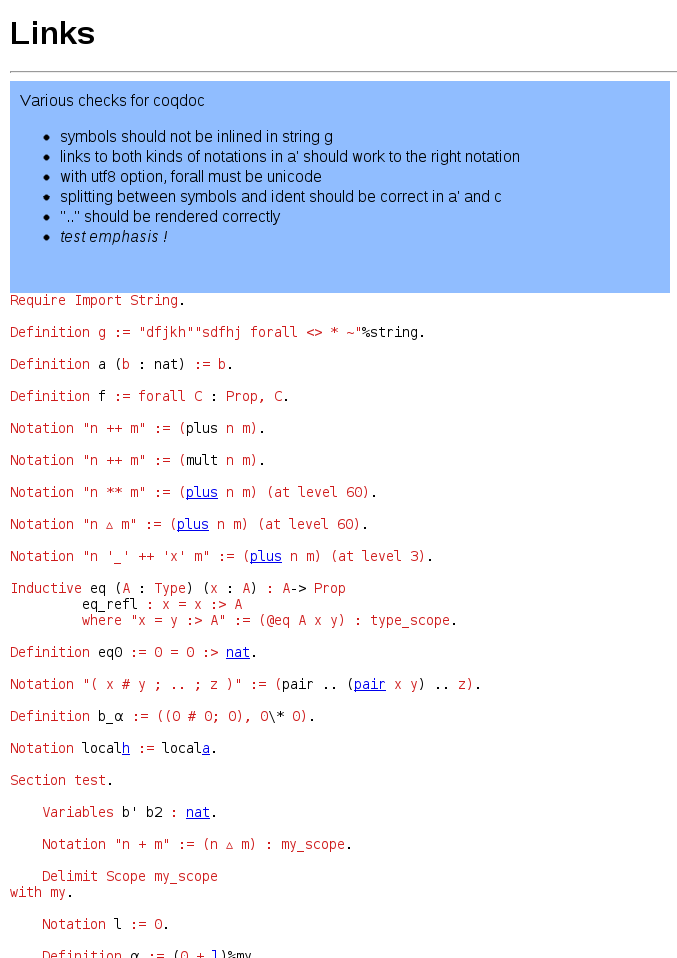
\includegraphics[scale=0.7]{data/html.png}}
  \caption{Exemple de rendu en HTML}
  \end{figure}
  \clearpage
  \begin{figure}
  \fbox{
  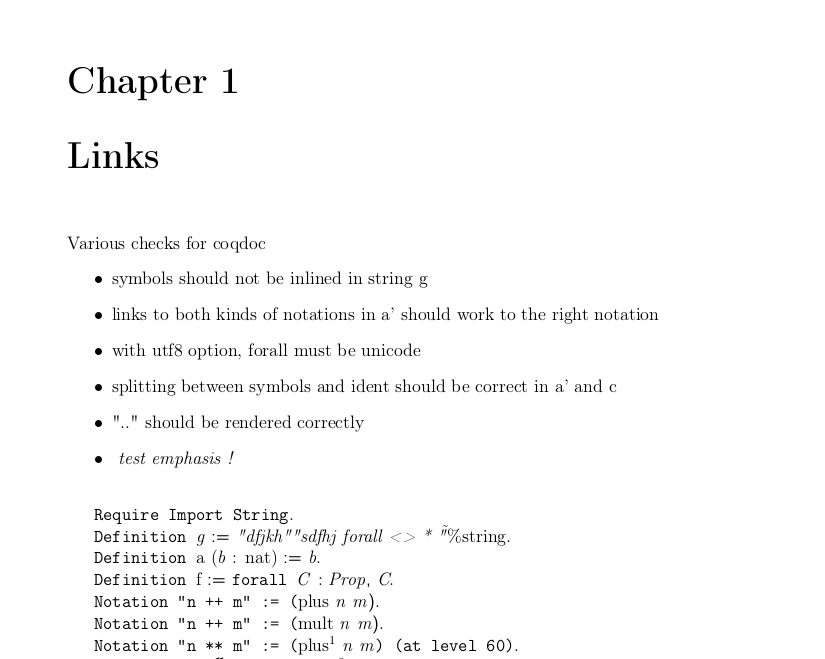
\includegraphics[scale=0.7]{data/pdf.png}}
  \caption{Exemple de rendu en LateX}
  \end{figure}
  \clearpage
  %% FIXME: faire des copies d'écran pour le HTML et inclure le pdf

\end{document}
